\documentclass[12pt,a4paper]{article}
\usepackage[utf8]{inputenc}
\usepackage[left=1in,right=1in,top=1in,bottom=1.25in]{geometry}
\usepackage{times}
\usepackage{graphicx}
\usepackage{booktabs}
\usepackage{tabularx}
\usepackage{array}
\usepackage{tikz}
\usetikzlibrary{shapes.geometric, arrows.meta, positioning}
\usepackage{fancyhdr}
\usepackage{hyperref}

\pagestyle{fancy}
\fancyhf{}
\renewcommand{\headrulewidth}{0pt}
\renewcommand{\footrulewidth}{1pt}
\lfoot{\textcopyright\ Department of Computer Science\\Faculty of Computing \& IT\\University of Gujrat}
\rfoot{\thepage}

\begin{document}

% =========================================================================
% PAGE 1: TITLE PAGE
% =========================================================================
\begin{titlepage}
\centering
{\fontsize{17.2pt}{22pt}\selectfont \textbf{Department of Computer Science}}\\[6pt]
{\fontsize{17.2pt}{22pt}\selectfont \textbf{University of Gujrat}}\\[18pt]


\includegraphics[width=6.5cm,keepaspectratio]{uog_logo.png}\\[28pt]

{\fontsize{18pt}{23pt}\selectfont \textbf{DeepTrace: An Explainable Multi-Agent AI System and Computer Vision Pipeline for Digital Financial Document Forensics and Tampering Detection}}\\[32pt]

\renewcommand{\arraystretch}{1.5}
\begin{tabular}{|p{6.5cm}|p{3.5cm}|}
\hline
\centering \textbf{Muhammad Shaheer Ul Hassan} & \centering \textbf{23011519-010} \tabularnewline
\hline
\centering \textbf{Samreen Aslam} & \centering \textbf{23011519-026} \tabularnewline
\hline
\centering \textbf{Mahnoor Sajid} & \centering \textbf{23011519-062} \tabularnewline
\hline
\end{tabular}\\[36pt]

{\fontsize{13pt}{16pt}\selectfont \textbf{Supervised By:}}\\[6pt]
{\fontsize{15pt}{18pt}\selectfont \textbf{Dr. Muhammad Sami Ullah}}\\[18pt]

\vfill
\end{titlepage}

% =========================================================================
% PAGE 2: DECLARATION
% =========================================================================
\newpage
\setcounter{page}{1}

\noindent{\fontsize{14.3pt}{18pt}\selectfont \textbf{DECLARATION}}\\[18pt]

\noindent I certify that project title \textbf{DeepTrace: An Explainable Multi-Agent AI System and Computer Vision Pipeline for Digital Financial Document Forensics and Tampering Detection} is under my supervision with students of \textbf{BS Computer Science}, Faculty of Computing \& Information Technology, University of Gujrat, Pakistan, worked under my supervision.\\[70pt]

\noindent\rule{6.2cm}{0.75pt}\\[8pt]
\noindent \textbf{Dr. Muhammad Sami Ullah}\\
Department of Computer Science\\
Faculty of Computing \& Information Technology\\
University of Gujrat, Punjab, Pakistan.\\
Email: supervisor@uog.edu.pk\\
Dated: September 21, 2026

% =========================================================================
% PAGE 3: ABSTRACT, INTRODUCTION, PROJECT TITLE
% =========================================================================
\newpage
\setcounter{page}{1}

\begin{center}
{\fontsize{17.2pt}{22pt}\selectfont \textbf{Final Year Project Proposal}}\\[16pt]
\end{center}

\noindent{\fontsize{14.3pt}{18pt}\selectfont \textbf{Abstract}}\\[8pt]
Digital fraud involving forged and manipulated financial documents---such as altered bank account statements, falsified salary slips, tampered utility bills, and counterfeit tax certificates---poses severe economic and compliance risks to banking, microfinance, and regulatory institutions. Contemporary forensic approaches either rely on slow manual inspection or opaque deep learning models that fail to produce legally admissible, explainable evidence. This project presents \textbf{DeepTrace: An Explainable Multi-Agent AI System and Computer Vision Pipeline for Digital Financial Document Forensics and Tampering Detection}, an enterprise-grade platform compliant with the State Bank of Pakistan (SBP) Frameworks, Electronic Transactions Ordinance (ETO 2002), PECA 2016, and NIST SP 800-86 forensic standards. DeepTrace employs a Tri-Pillar Architecture integrating deterministic rule verification (Lakh/Crore balance reconciliations, PK-IBAN MOD-97 check digits, and PDF incremental update trees), computer vision forensics (Error Level Analysis at $Q=95$, copy-move forgery detection, and font baseline displacement mapping), and a LangGraph-coordinated Multi-Agent AI Swarm enforcing a strict zero-hallucination evidence policy. The system features a containerized FastAPI backend, an interactive web dashboard, and a dedicated Flutter mobile application for on-field document capture and rapid forensic inspection. Experimental evaluations demonstrate sub-3.5-second processing latency and verifiable pixel-level evidence localization.\\[14pt]

\noindent{\fontsize{14.3pt}{18pt}\selectfont \textbf{1\quad Introduction}}\\[8pt]
This proposal defines the functional specifications, technical architecture, deployment topology, and development roadmap for DeepTrace. Financial institutions and government agencies process millions of digital records annually, yet remain highly vulnerable to sophisticated digital tampering executed via desktop image editors and generative tools. DeepTrace addresses these critical vulnerabilities by combining deterministic mathematical validation with advanced computer vision and an autonomous multi-agent reasoning swarm, bridging the gap between automated fraud detection and court-admissible digital forensics.\\[14pt]

\noindent{\fontsize{14.3pt}{18pt}\selectfont \textbf{2\quad Project Title}}\\[8pt]
\textbf{DeepTrace: An Explainable Multi-Agent AI System and Computer Vision Pipeline for Digital Financial Document Forensics and Tampering Detection.}

% =========================================================================
% PAGE 4: PROJECT OVERVIEW, TARGETED AUDIENCE, GOALS
% =========================================================================
\newpage
\noindent{\fontsize{14.3pt}{18pt}\selectfont \textbf{3\quad Project Overview}}\\[8pt]
Traditional financial verification systems rely on fragmented manual checks or unexplainable black-box machine learning models that fail to pinpoint exact fraudulent alterations. DeepTrace establishes an end-to-end digital forensic pipeline governed by SHA-256 cryptographic locking and immutable audit logs. The platform ingests electronic PDFs and high-resolution document scans, subjecting each artifact to multi-stage forensic scrutiny: PDF object-tree decompilation, sub-pixel font baseline analysis, Error Level Analysis (ELA at $Q=95$), copy-move forgery detection, and mathematical balance reconciliations. A LangGraph-coordinated swarm of four specialized LLM agents (Structural, Visual, Semantic, and Lead Investigator) synthesizes multi-modal findings into an explainable forensic case manifest, eliminating false accusations and providing legally defensible audit trails accessible across web and mobile platforms.\\[14pt]

\noindent{\fontsize{14.3pt}{18pt}\selectfont \textbf{4\quad Targeted Audience}}\\[8pt]
The primary users and institutional beneficiaries of this system include:
\begin{itemize}
    \setlength\itemsep{4pt}
    \item \textbf{Commercial Banks \& Microfinance Institutions:} Credit risk officers and underwriting teams vetting applicant bank statements, salary slips, and collateral proofs for loan originations.
    \item \textbf{Fintechs \& Digital Lending Platforms:} Fast-growing micro-lenders requiring automated REST API endpoints (\texttt{/api/v1/verify}) for real-time document validation during digital onboarding.
    \item \textbf{Law Enforcement \& Forensic Laboratories:} Cybercrime investigators (FIA, Police) and judicial prosecutors requiring tamper-evident chain of custody and court-admissible forensic packages.
    \item \textbf{Corporate HR \& Visa Verification Agencies:} Screening teams verifying educational credentials, income certificates, and employer tax declarations against institutional impersonation.
\end{itemize}

\vspace{6pt}
\noindent{\fontsize{14.3pt}{18pt}\selectfont \textbf{5\quad Project Goals \& Objectives}}\\[8pt]
\noindent\textbf{Goals:}
\begin{itemize}
    \setlength\itemsep{3pt}
    \item Modernize financial compliance workflows by eliminating manual document vetting vulnerabilities.
    \item Deliver an explainable, tri-pillar forensic framework fusing deterministic rules, computer vision, and multi-agent AI.
    \item Provide unified cross-platform accessibility via an enterprise FastAPI backend, Next.js web dashboard, and Flutter mobile scanner.
    \item Enforce strict chain of custody and evidentiary immutability conforming to SBP, PECA 2016, and ETO 2002 regulations.
\end{itemize}

% =========================================================================
% PAGE 5: MEASURABLE OBJECTIVES, APPLICATION ARCHITECTURE & DIAGRAM
% =========================================================================
\newpage
\noindent\textbf{Measurable Objectives:}
\begin{itemize}
    \setlength\itemsep{4pt}
    \item Deliver an automated multi-stage forensic analysis pipeline executing full document evaluation in under 3.5 seconds for vector PDFs and under 6.0 seconds for high-resolution 300 DPI scans.
    \item Achieve over 96\% detection accuracy across synthetic and copy-move forgery benchmarks with sub-pixel bounding box localization (Intersection over Union $\ge 0.85$).
    \item Guarantee 100\% deterministic detection of mathematical balance inconsistencies, IBAN checksum anomalies (MOD-97), and incremental PDF revision tampering.
    \item Enforce zero-hallucination agentic reporting by strictly constraining LangGraph LLM synthesis to verified forensic manifests with full cryptographic SHA-256 evidence anchoring.
    \item Deploy a containerized microservice architecture sustaining 50+ concurrent verification requests with sub-second database query latency through optimized PostgreSQL partial indexing and Redis caching.
\end{itemize}

\vspace{10pt}
\noindent{\fontsize{14.3pt}{18pt}\selectfont \textbf{6\quad Application Architecture}}\\[8pt]
The system employs an enterprise Three-Tier Microservice Architecture (Client, Application/Forensic, and Data/Storage tiers) interconnected via secure RESTful APIs and real-time WebSockets.\\[14pt]

\begin{center}
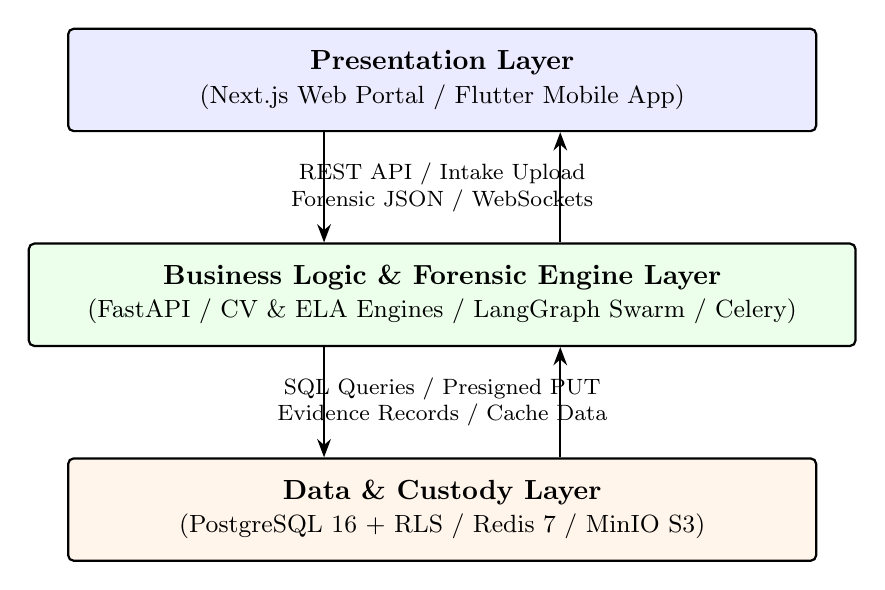
\begin{tikzpicture}[
    box/.style={draw, rectangle, rounded corners=2pt, minimum width=9.5cm, minimum height=1.3cm, align=center, line width=0.8pt},
    arr/.style={-{Stealth[scale=1.0]}, line width=0.8pt}
]
    % Tier 1
    \node[box, fill=blue!8] (tier1) {
        \textbf{Presentation Layer}\\
        \small (Next.js Web Portal / Flutter Mobile App)
    };

    % Tier 2
    \node[box, fill=green!8, minimum width=10.5cm, below=1.4cm of tier1] (tier2) {
        \textbf{Business Logic \& Forensic Engine Layer}\\
        \small (FastAPI / CV \& ELA Engines / LangGraph Swarm / Celery)
    };

    % Tier 3
    \node[box, fill=orange!8, below=1.4cm of tier2] (tier3) {
        \textbf{Data \& Custody Layer}\\
        \small (PostgreSQL 16 + RLS / Redis 7 / MinIO S3)
    };

    % Arrows 1
    \draw[arr] ([xshift=-1.5cm]tier1.south) -- ([xshift=-1.5cm]tier2.north);
    \draw[arr] ([xshift=1.5cm]tier2.north) -- ([xshift=1.5cm]tier1.south);
    \node[font=\footnotesize, align=center] at ([yshift=0.7cm]tier2.north) {REST API / Intake Upload\\Forensic JSON / WebSockets};

    % Arrows 2
    \draw[arr] ([xshift=-1.5cm]tier2.south) -- ([xshift=-1.5cm]tier3.north);
    \draw[arr] ([xshift=1.5cm]tier3.north) -- ([xshift=1.5cm]tier2.south);
    \node[font=\footnotesize, align=center] at ([yshift=0.7cm]tier3.north) {SQL Queries / Presigned PUT\\Evidence Records / Cache Data};
\end{tikzpicture}
\end{center}

% =========================================================================
% PAGE 6: HARDWARE & SOFTWARE SPEC, ESTIMATED COST, TOOLS & TECHNOLOGIES
% =========================================================================
\newpage
\noindent{\fontsize{14.3pt}{18pt}\selectfont \textbf{7\quad Hardware and Software Specification}}\\[8pt]
\begin{table}[h]
\centering
\small
\begin{tabularx}{\textwidth}{lX}
\toprule
\textbf{Category} & \textbf{Specification} \\
\midrule
\textbf{Development Machine} & Intel Core i7 / AMD Ryzen 7 (16GB ECC RAM, 512GB NVMe SSD) \\
\textbf{Operating System} & Ubuntu 24.04 LTS (Production Server) / Windows 11 Dev Environment \\
\textbf{Virtualization/Hosting} & Docker Engine \& Docker Compose Multi-Container Stack, Caddy Proxy \\
\textbf{Database Management} & PostgreSQL 16 (pgcrypto, pg\_trgm, btree\_gin, RLS) + Prisma ORM + Redis 7 \\
\textbf{Mobile Runtime} & Flutter 3.x / Dart 3.x (Android SDK 34+, iOS 17+) with Physical Test Devices \\
\textbf{Version Control} & Git (GitHub Enterprise / Repository with Automated CI/CD Actions) \\
\bottomrule
\end{tabularx}
\end{table}

\noindent{\fontsize{14.3pt}{18pt}\selectfont \textbf{8\quad Estimated Cost}}\\[8pt]
\begin{table}[h]
\centering
\small
\begin{tabularx}{\textwidth}{Xcr}
\toprule
\textbf{Item Description} & \textbf{Quantity} & \textbf{Estimated Cost (PKR)} \\
\midrule
Domain Name (.edu.pk / .com with SSL) & 1 & 5,000 \\
Cloud Hosting VPS Server (1 Year Production Tier) & 1 & 32,000 \\
LLM API Inference Credits \& Cloud Storage Benchmarking & - & 12,000 \\
Mobile App Testing \& Play Store Developer Licensing & 1 & 8,500 \\
Hardware Upgrades, Storage Contingency \& Testing Supplies & - & 7,500 \\
\midrule
\textbf{Total Estimated Cost} & & \textbf{65,000} \\
\bottomrule
\end{tabularx}
\end{table}

\noindent{\fontsize{14.3pt}{18pt}\selectfont \textbf{9\quad Tools and Technologies Used}}\\[8pt]
\begin{itemize}
    \setlength\itemsep{3pt}
    \item \textbf{FastAPI (Python 3.12):} Delivers an asynchronous, high-concurrency backend API with native Pydantic v2 data validation, OpenAPI self-documentation, and low-latency non-blocking forensic task dispatching.
    \item \textbf{Flutter \& Dart:} Provides a responsive, high-performance cross-platform mobile application for Android and iOS featuring hardware-accelerated camera intake, real-time edge scanning, and offline case inspection.
    \item \textbf{PostgreSQL 16 \& Prisma ORM:} Enterprise relational database configured with Row-Level Security (RLS) policies for multi-tenancy, immutable audit logging triggers for legal compliance, and trigram fuzzy search indexes.
    \item \textbf{PyMuPDF \& OpenCV:} Executes low-level PDF parsing, vector font baseline extraction, copy-move forgery detection, glyph anomaly localization, and Error Level Analysis (ELA at $Q=95$).
    \item \textbf{LangGraph \& Multi-Agent Swarm:} Coordinates specialized forensic LLM agents (Structural, Visual, Semantic, Lead Investigator) bound to verified evidence manifests under a zero-hallucination policy.
    \item \textbf{Docker \& Caddy:} Encapsulates microservices into lightweight reproducible containers with automated SSL reverse-proxy routing and zero-downtime containerized deployments.
\end{itemize}

% =========================================================================
% PAGE 7: PROJECT MILESTONES & WORK DIVISION
% =========================================================================
\newpage
\noindent{\fontsize{14.3pt}{18pt}\selectfont \textbf{10\quad Project Milestones and Deliverables}}\\[6pt]
\noindent The project timeline spans 12 weeks, broken down into distinct development phases.\\[8pt]

\begin{center}
\textbf{\small FYP Development Timeline (Weeks)}\\[4pt]
\small
\begin{tabular}{|l|c|c|c|c|c|c|c|c|c|c|c|c|}
\hline
\textbf{Phase / Milestone} & \textbf{1} & \textbf{2} & \textbf{3} & \textbf{4} & \textbf{5} & \textbf{6} & \textbf{7} & \textbf{8} & \textbf{9} & \textbf{10} & \textbf{11} & \textbf{12} \\
\hline
Requirements Analysis \& SRS & \rule{12pt}{6pt} & \rule{12pt}{6pt} & & & & & & & & & & \\
\hline
Architecture \& UI/UX Design & & & \rule{12pt}{6pt} & \rule{12pt}{6pt} & & & & & & & & \\
\hline
Backend \& Forensic CV Pipeline & & & & \rule{12pt}{6pt} & \rule{12pt}{6pt} & \rule{12pt}{6pt} & \rule{12pt}{6pt} & & & & & \\
\hline
Flutter App \& Web Dashboard & & & & & & \rule{12pt}{6pt} & \rule{12pt}{6pt} & \rule{12pt}{6pt} & \rule{12pt}{6pt} & & & \\
\hline
Multi-Agent Swarm \& Testing & & & & & & & & & \rule{12pt}{6pt} & \rule{12pt}{6pt} & \rule{12pt}{6pt} & \\
\hline
Final Documentation \& Launch & & & & & & & & & & & \rule{12pt}{6pt} & \rule{12pt}{6pt} \\
\hline
\end{tabular}
\end{center}

\vspace{10pt}
\noindent{\fontsize{14.3pt}{18pt}\selectfont \textbf{11\quad Work Division Among Group Members}}\\[6pt]
\begin{table}[h]
\centering
\footnotesize
\begin{tabularx}{\textwidth}{p{3.5cm}X}
\toprule
\textbf{Team Member} & \textbf{Assigned Responsibilities} \\
\midrule
\textbf{Muhammad Shaheer Ul Hassan}\newline \textcolor{gray}{23011519-010} & 
\textbf{Backend Architecture, Forensic CV Engines, AI Swarm \& Cloud Deployment:}\newline
$\bullet$ \textit{Backend \& Database:} High-concurrency FastAPI microservices, Pydantic v2 schemas, PostgreSQL 16 schema with Prisma ORM, 19 Row-Level Security (RLS) policies, and immutable audit triggers.\newline
$\bullet$ \textit{Forensic CV Pipelines:} Error Level Analysis (ELA at $Q=95$), font baseline displacement mapping, and copy-move forgery detection using PyMuPDF and OpenCV.\newline
$\bullet$ \textit{Deterministic Checks \& Swarm:} Mathematical balance reconciliations, PK-IBAN MOD-97 check digits, and LangGraph Multi-Agent Swarm with zero-hallucination policy.\newline
$\bullet$ \textit{DevOps \& Security:} Docker multi-container stack, Caddy reverse proxy (auto-SSL), Redis caching, Celery task queue, S3/MinIO custody storage, and SBP/PECA compliance. \\
\midrule
\textbf{Samreen Aslam}\newline \textcolor{gray}{23011519-026} & 
\textbf{Cross-Platform Mobile Application, Intake Scanner \& UI/UX:}\newline
$\bullet$ \textit{Cross-Platform Client:} Developed native-speed Android and iOS mobile applications using Flutter 3.x and Dart.\newline
$\bullet$ \textit{Mobile Document Scanner:} Hardware-accelerated camera intake with real-time document boundary edge detection, perspective correction, and multi-page capture.\newline
$\bullet$ \textit{Interactive Forensic Viewer:} Zoomable high-DPI document canvas with pixel-level bounding box overlays, visual diff highlighting, and ELA heatmap inspection.\newline
$\bullet$ \textit{Case Management \& Sync:} Mobile case dashboard with status filters, push notifications on pipeline completion, biometric auth, and presigned S3 evidence upload streams. \\
\midrule
\textbf{Mahnoor Sajid}\newline \textcolor{gray}{23011519-062} & 
\textbf{Software Requirements Specification (SRS), System Modeling \& SQA:}\newline
$\bullet$ \textit{SRS Authoring:} Formulated comprehensive Software Requirements Specification (SRS) strictly conforming to IEEE Std 830-1998 guidelines.\newline
$\bullet$ \textit{System Modeling:} Designed complete UML behavioral and structural models (Use Case, Class, Sequence, Activity diagrams, and ERD schemas).\newline
$\bullet$ \textit{Legal \& Regulatory Compliance:} Conducted compliance mapping for PECA 2016, Electronic Transactions Ordinance (ETO 2002), SBP digital onboarding frameworks, and NIST SP 800-86.\newline
$\bullet$ \textit{QA \& Final Deliverables:} SQA test plan, User Acceptance Testing (UAT) verification trace matrices, final project proposal, and formal evaluation documentation. \\
\bottomrule
\end{tabularx}
\end{table}

\end{document}
